%%%%%%%%%%%%%%%%%%%%%%%%%%%%%%%%%%%%%%%%%%%%%%%%%%%%%%%%%%%%%%%
%
%
%   This file is included in Registration.tex
%
%   Lablels and section entries are defined in that file.
%
%
%
%%%%%%%%%%%%%%%%%%%%%%%%%%%%%%%%%%%%%%%%%%%%%%%%%%%%%%%%%%%%%%%

 
\begin{figure} \center
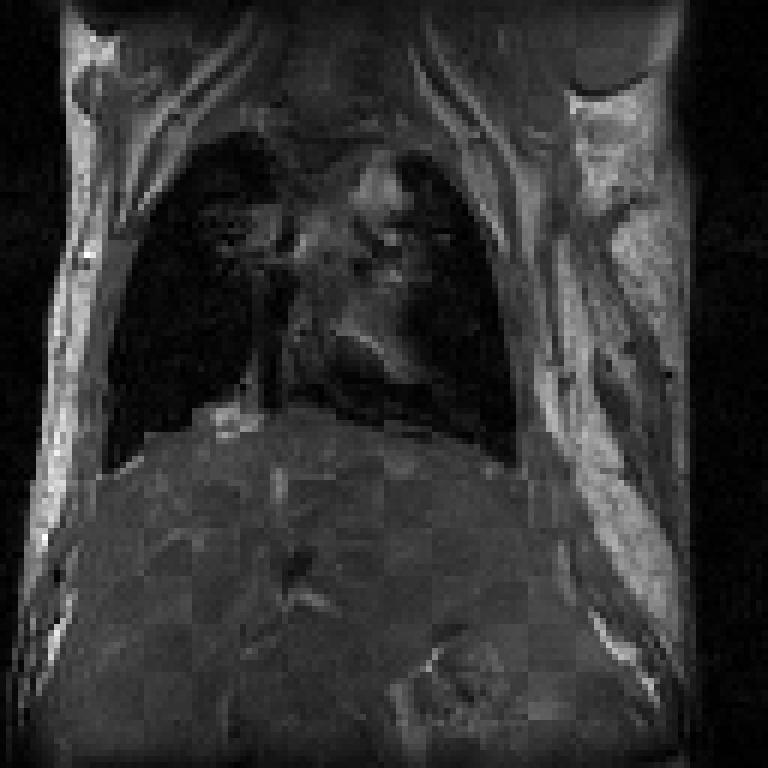
\includegraphics[width=0.44\textwidth]{DeformableRegistration1CheckerboardBefore.eps}
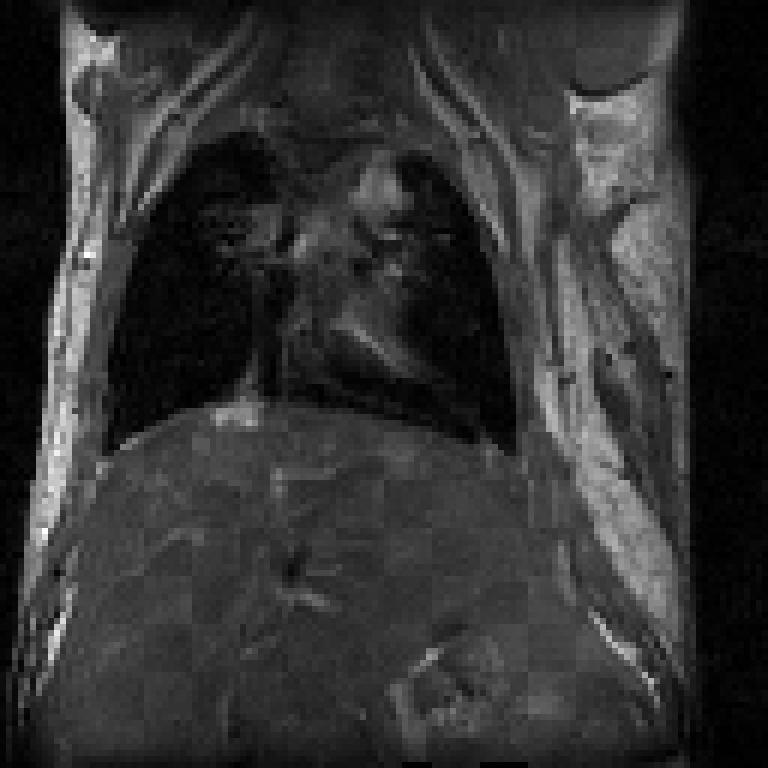
\includegraphics[width=0.44\textwidth]{DeformableRegistration1CheckerboardAfter.eps}
\itkcaption[FEM-based deformable registration results]{Checkerboard comparisons
before and after FEM-based deformable registration.}
\label{fig:DeformableRegistration1Output}
\end{figure}

\ifitkFullVersion
\input{DeformableRegistration1.tex}
\fi

Figure \ref{fig:DeformableRegistration1Output} presents the results of
the FEM-based deformable registration applied to two time-separated
slices of a living mouse dataset.  Checkerboard comparisons of the two
images are shown before registration (left) and after registration
(right).  Both images were acquired from the same living mouse, the
first after inspiration of air into the lungs and the second after
exhalation.  Deformation occurs due to the elastic recoil of the lung
tissue and the relaxation of the diaphragm.

The following is a documented sample parameter file that can be used with this
deformable registration example.  This example demonstrates the setup of a
basic registration problem that does not use multi-resolution strategies.  As a
result, only one value for the parameters between \texttt{(\# of pixels per
element)} and \texttt{(maximum iterations)} is necessary.  In order to use a
multi-resolution strategy, you would have to specify values for those
parameters at each level of the pyramid.

\verbatiminput{FiniteElementRegistrationParameters1.txt}


